\documentclass[11pt,a4paper]{article}

\usepackage[margin=1in,headheight=15pt,headsep=24pt,footskip=28pt]{geometry}
\usepackage[default]{sourcesanspro}
\usepackage{setspace}
\usepackage{xcolor}
\usepackage{titlesec}
\usepackage{fancyhdr}
\usepackage{lastpage}
\usepackage{microtype}
\usepackage{graphicx}
\usepackage{booktabs}
\usepackage{array}
\usepackage{float}
\usepackage[section]{placeins}
\usepackage[hidelinks]{hyperref}
\usepackage[numbers,sort&compress]{natbib}
\renewcommand{\bibsection}{\unnumberedheading{References}}

\setstretch{1.35}
\setlength{\parindent}{0pt}
\setlength{\parskip}{8pt}
\raggedbottom

\titleformat{\section}{\fontsize{14}{16.5}\selectfont\bfseries}{\thesection}{1em}{}
\titlespacing*{\section}{0pt}{6pt}{8pt}
\titleformat{\subsection}{\fontsize{12.5}{15}\selectfont\bfseries}{\thesubsection}{1em}{}
\titlespacing*{\subsection}{0pt}{4pt}{2pt}

\newcommand{\unnumberedheading}[1]{%
  \par\vspace{2pt}{\fontsize{14}{16.5}\selectfont\bfseries #1\par}\vspace{6pt}%
}
\newcommand{\reporttitle}[1]{%
  {\fontsize{16}{19}\selectfont\bfseries #1\par}\vspace{12pt}%
}

\pagestyle{fancy}
\fancyhf{}
\renewcommand{\headrulewidth}{0pt}
\renewcommand{\footrulewidth}{0pt}
\fancyhead[L]{\fontsize{9}{11}\selectfont II2202, Autumn 2026, Period 1}
\fancyhead[C]{\fontsize{9}{11}\selectfont Quantitative exercise}
\fancyhead[R]{\fontsize{9}{11}\selectfont 21 September 2026}
\fancyfoot[R]{\fontsize{8.5}{10}\selectfont \thepage\ (\pageref{LastPage})}

\begin{document}

\reporttitle{Predicting Exoplanet Radius from Planetary and Stellar Properties}
\unnumberedheading{Authors}
Lorenzo Deflorian <ldef@kth.se>\par
Juozas Skarbalius <juozas@kth.se>\par

\section{Dataset and Research Question}

This exercise asks: \emph{How accurately can the radius of a transiting exoplanet be predicted from its mass, orbit, equilibrium temperature, and host-star properties?} We use the Planetary Systems Composite Parameters table from the NASA Exoplanet Archive, which integrates published measurements of confirmed planets and their host stars~\cite{akeson2013archive,nasaarchive2026}. The archive is continuously updated, so we saved the queried CSV and its checksum rather than depending on a live result.

The snapshot contains 6,316 confirmed planets with a reported radius. We restricted the analysis to transit discoveries because this gives a more consistent radius-detection context. Of the 4,707 transit planets, 2,974 had masses whose archive provenance was ``M-R relationship.'' Those masses were inferred from a mass--radius relationship; using them to predict radius would leak information from the outcome into an input. We therefore retained only the 1,693 entries whose provenance was ``Mass.'' Removing 23 rows missing equilibrium temperature or stellar metallicity gave a final sample of 1,670 planets in 1,304 host systems. Table~\ref{tab:selection} makes every selection step explicit.

\begin{table}[tbp]
  \centering
  \small
  \begin{tabular}{>{\raggedright\arraybackslash}p{7.9cm}r}
    \toprule
    Selection step & Planets remaining \\
    \midrule
    Confirmed planets with a reported radius & 6,316 \\
    Discovered with the transit method & 4,707 \\
    Mass provenance recorded as ``Mass'' & 1,693 \\
    Complete values, with positive log-transformed quantities & 1,670 \\
    \bottomrule
  \end{tabular}
  \caption{Sample construction from the archive snapshot.}
  \label{tab:selection}
\end{table}

\section{Variables and Expected Properties}

The term \emph{independent variable} describes predictor role; it does not mean that the catalog variables are experimentally manipulated or mutually independent. Astronomical catalogs are observational and affected by which planets can be detected and characterized. Table~\ref{tab:variables} records our expectations before fitting a model.

\begin{table}[H]
  \centering
  \small
  \begin{tabular}{>{\raggedright\arraybackslash}p{2.7cm}>{\raggedright\arraybackslash}p{2.4cm}>{\raggedright\arraybackslash}p{7.2cm}}
    \toprule
    Variable & Role and unit & Expected properties \\
    \midrule
    Planet radius & Dependent, Earth radii & Positive and continuous. Multiple planetary regimes should make its distribution non-normal and its relationship with mass nonlinear. \\
    Planet mass & Independent, Earth masses & Positive and strongly right-skewed. Expected to be the most informative predictor, with radius increasing rapidly for smaller planets and flattening for gas giants~\cite{chen2017massradius}. \\
    Orbital period & Independent, days & Positive and right-skewed. Its association may reflect irradiation and transit-selection effects rather than a direct causal influence. \\
    Equilibrium temperature & Independent, kelvin & Positive. Hotter gas planets may be inflated, but temperature is also related to orbit and stellar properties. \\
    Stellar mass & Independent, solar masses & Positive. It may be associated with planet populations and is correlated with other stellar quantities. \\
    Stellar metallicity & Independent, dex & May be negative or positive because it is logarithmic relative to the Sun. We expected a weaker population-level association. \\
    \bottomrule
  \end{tabular}
  \caption{Dependent and independent variables and their expected properties.}
  \label{tab:variables}
\end{table}

Stellar radius was available but excluded from the predictors because a transit-derived absolute planet radius depends on the adopted stellar radius. Planet density was also excluded because it is calculated using planet mass and radius. These decisions reduce direct mathematical leakage into the dependent variable.

\section{Preprocessing and Analysis Method}

The archive CSV was loaded with pandas. The script verified the exact schema, unique planet names, missingness, and positivity of quantities that were later logarithmically transformed. There were no duplicate planet names or nonpositive values in the selected sample. Complete-case removal affected only 23 of 1,693 otherwise eligible planets (1.4\%): four equilibrium temperatures and 22 stellar metallicities were missing, with three rows missing both.

Exploratory analysis used summary statistics, distributions, scatterplots, and Spearman rank correlations. Spearman correlation was selected because mass and period were extremely skewed and the expected relationships were nonlinear. Before modelling, planet radius, planet mass, orbital period, and equilibrium temperature were transformed to base-10 logarithms. This reduces the leverage of extreme values and lets the linear model represent multiplicative relationships.

Three models were compared. A median-only model supplied a no-information baseline. Multiple linear regression fitted one additive plane in log space. A random-forest regressor~\cite{breiman2001random} represented nonlinearities and interactions without requiring a single physical equation. Principal component analysis was not selected because there is a defined dependent variable and supervised regression directly addresses the question; components that explain predictor variance do not necessarily predict radius.

Evaluation used ten-fold grouped cross-validation implemented with scikit-learn~\cite{pedregosa2011scikit}. All planets sharing a host star were assigned to the same fold, preventing shared stellar measurements from appearing in both training and test data. Performance measures were RMSE and MAE in Earth radii, $R^2$, and log-scale RMSE in dex. Each planet received one out-of-fold prediction. A 5,000-resample host-cluster bootstrap estimated uncertainty in the RMSE difference between models. Held-out permutation importance measured the increase in log-RMSE after shuffling one predictor. Finally, host-grouped five-fold learning curves examined whether adding observations continued to lower error.

\section{Results}

\subsection{Exploratory Data Analysis}

Planet radius ranged from 0.31 to 25.00 Earth radii, with mean 7.89, standard deviation 5.81, and median 6.85. The histogram in Figure~\ref{fig:eda}(a) contains a concentration of small planets and another broad concentration around giant-planet sizes, so a single normal distribution is inappropriate. Planet mass was highly right-skewed: its median was 65.74 Earth masses, while its mean was 325.10 and maximum was 8,899.20. Orbital period was even more skewed, with median 5.40 days and maximum 3,650 days. These properties supported the planned logarithmic transformations.

\begin{table}[tbp]
  \centering
  \small
  \begin{tabular}{lrrrrr}
    \toprule
    Variable & Mean & SD & Minimum & Median & Maximum \\
    \midrule
    Planet radius ($R_\oplus$) & 7.89 & 5.81 & 0.31 & 6.85 & 25.00 \\
    Planet mass ($M_\oplus$) & 325.10 & 795.16 & 0.07 & 65.74 & 8,899.20 \\
    Orbital period (days) & 23.07 & 112.20 & 0.18 & 5.40 & 3,650.00 \\
    Equilibrium temperature (K) & 1,068.90 & 519.65 & 134.40 & 980.10 & 3,921.00 \\
    Stellar mass ($M_\odot$) & 0.98 & 0.32 & 0.09 & 0.98 & 2.78 \\
    Stellar metallicity (dex) & 0.05 & 0.19 & -0.72 & 0.05 & 0.79 \\
    \bottomrule
  \end{tabular}
  \caption{Descriptive statistics for the 1,670-planet model sample.}
  \label{tab:descriptive}
\end{table}

Figure~\ref{fig:eda}(b) confirms the expected nonlinear mass--radius relationship. Median radius grows across the low- and intermediate-mass bins, then becomes nearly flat for giant planets. Panel (c) shows two partly overlapping populations rather than one simple temperature trend. The unadjusted Spearman correlations in panel (d) were 0.802 for planet mass, 0.568 for stellar mass, 0.549 for equilibrium temperature, 0.246 for stellar metallicity, and $-0.257$ for orbital period. Their directions largely matched our expectations, but these bivariate associations combine physical relationships with catalog selection. They are not causal effects.

\begin{figure}[tbp]
  \centering
  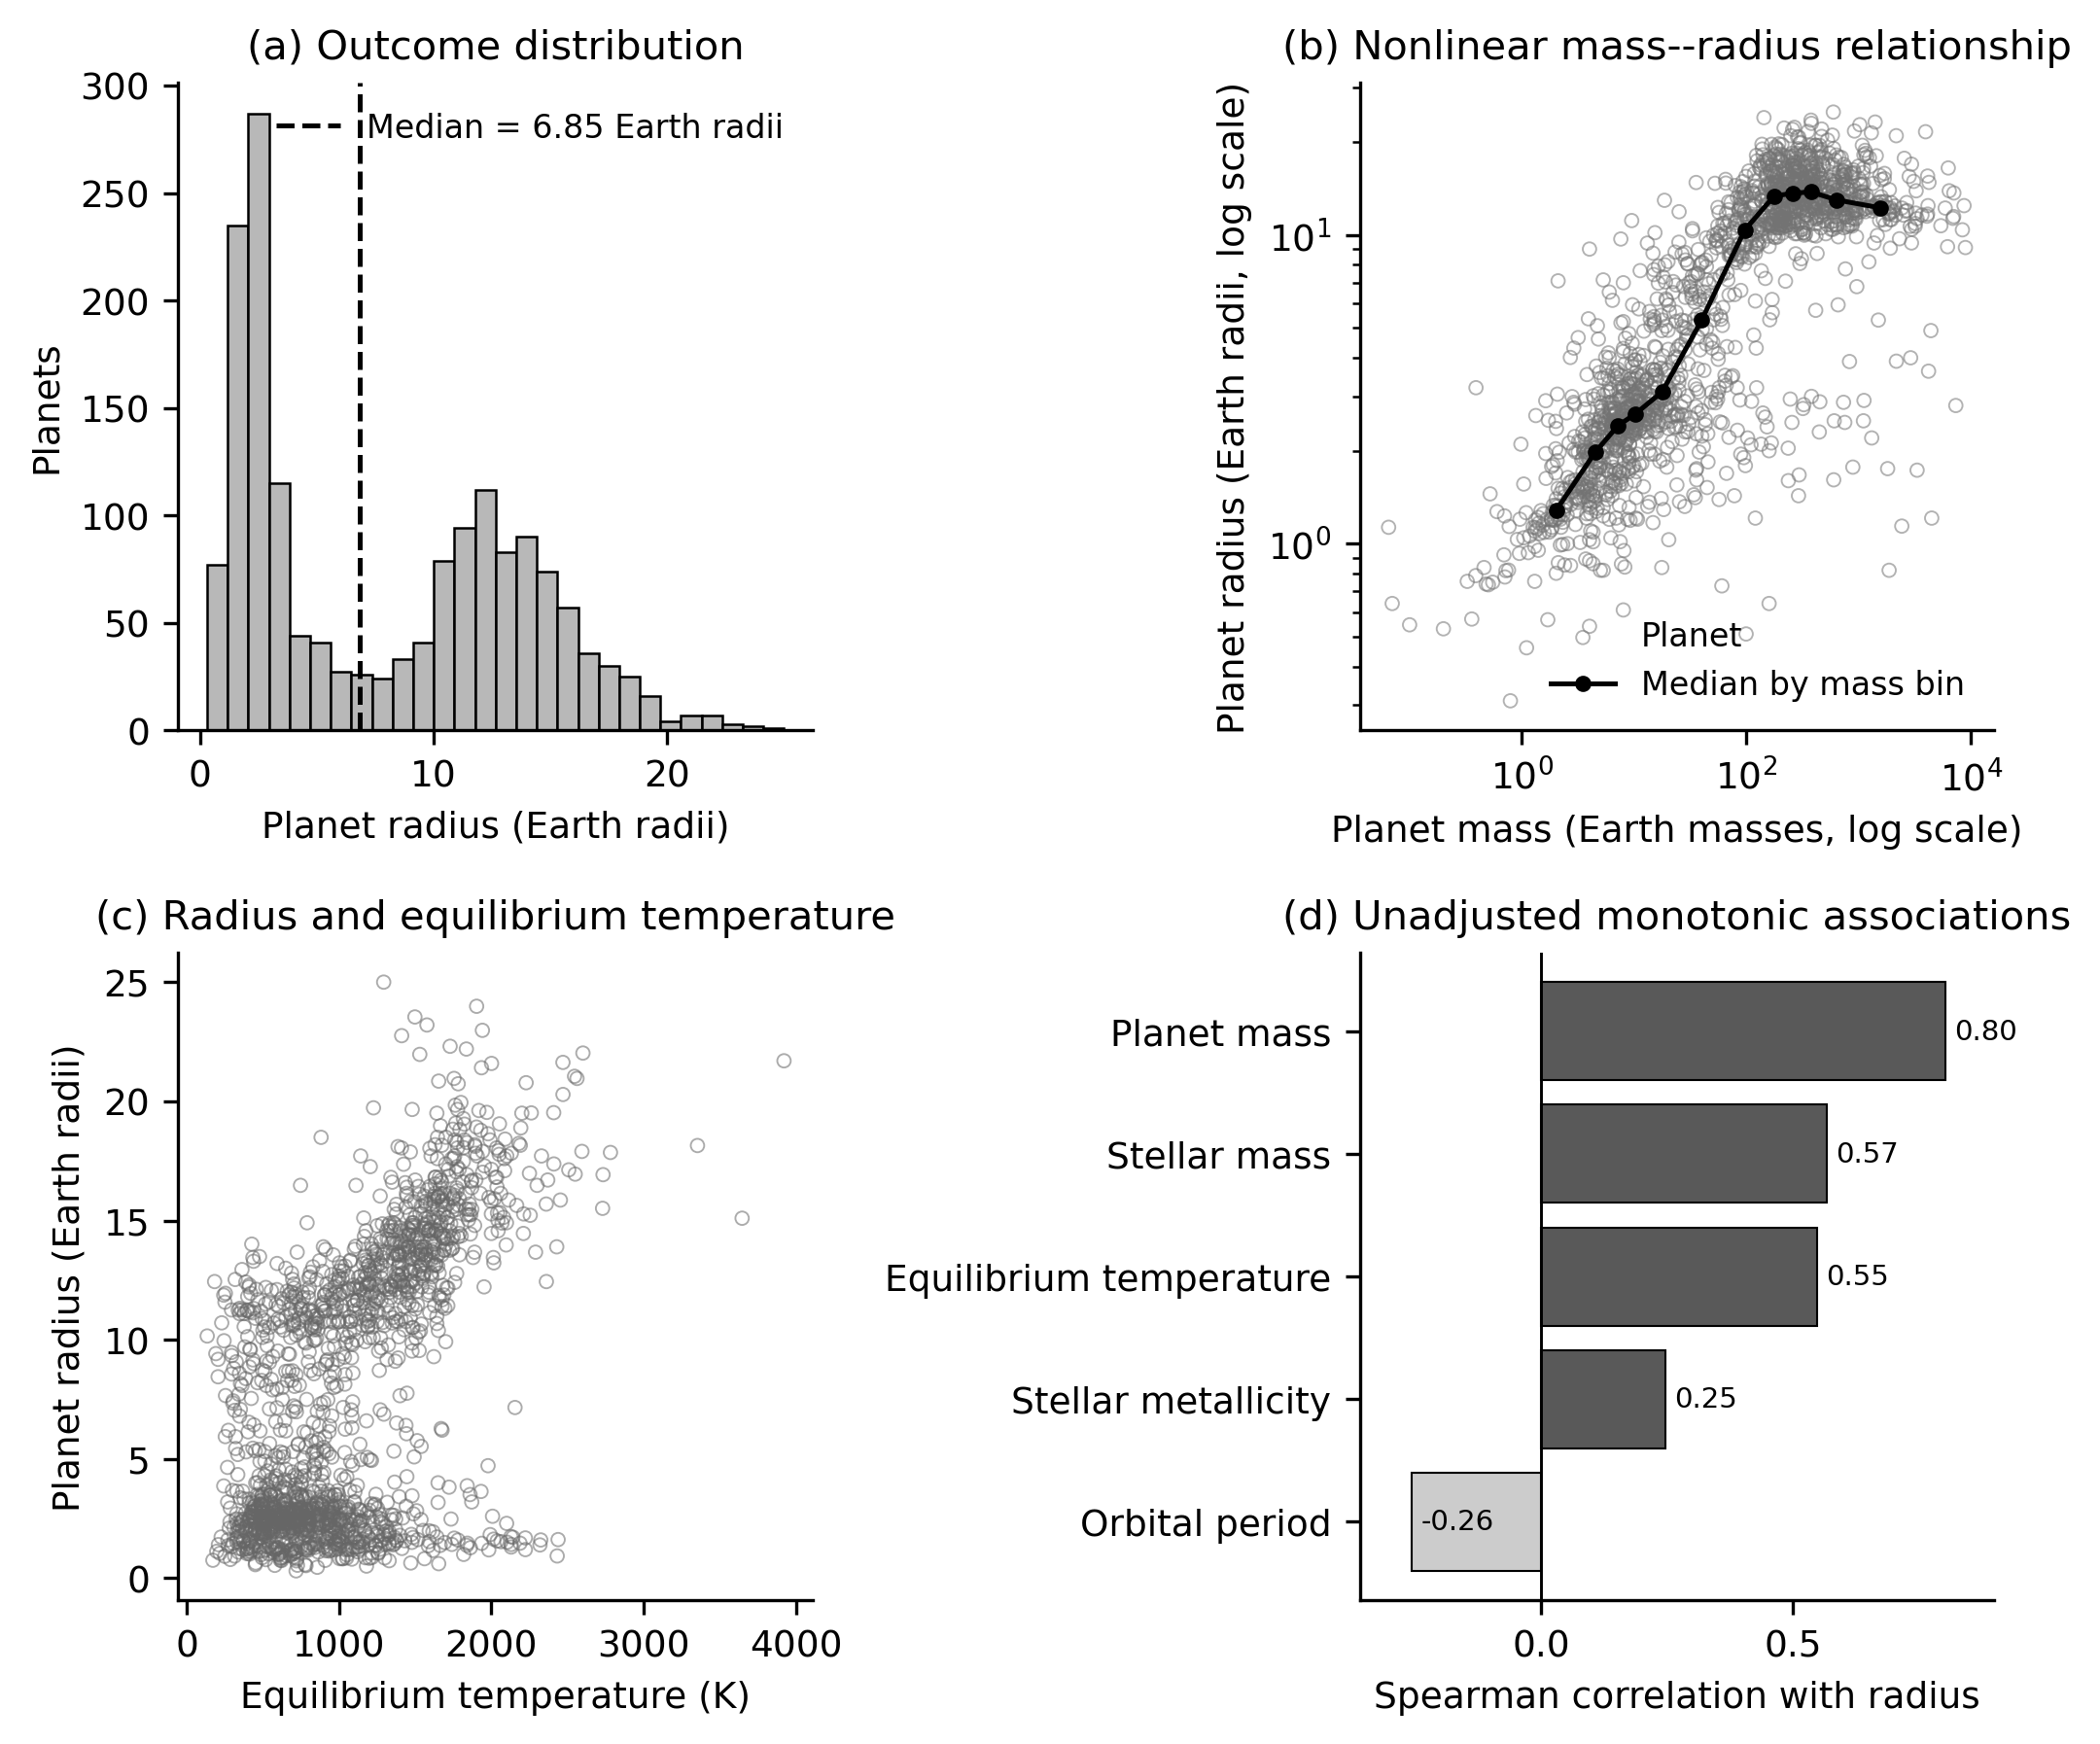
\includegraphics[width=\textwidth]{figures/exploratory_analysis.pdf}
  \caption{Exploratory analysis. Hollow points, line styles, gray levels, and direct numeric labels keep the plots interpretable without color.}
  \label{fig:eda}
\end{figure}

\subsection{Predictive Models}

Table~\ref{tab:models} shows that both fitted models improved substantially on the median baseline. The log-linear model attained a mean held-out RMSE of 4.18 Earth radii and explained 47.8\% of test variance. The random forest reduced mean RMSE to 2.40 Earth radii and explained 82.6\%. Pooled out-of-fold RMSEs were 4.19 and 2.42 Earth radii, respectively. Their reduction was 1.77 Earth radii; the host-cluster bootstrap 95\% interval was 1.50--2.03 Earth radii. Figure~\ref{fig:predictions} shows that the forest follows the small-, intermediate-, and giant-planet regimes more closely, whereas one log-linear surface systematically compresses the relationship.

\begin{table}[tbp]
  \centering
  \small
  \begin{tabular}{lrrrr}
    \toprule
    Model & RMSE ($R_\oplus$) & MAE ($R_\oplus$) & $R^2$ & Log-RMSE (dex) \\
    \midrule
    Median baseline & $5.91 \pm 0.18$ & $5.30 \pm 0.16$ & $-0.042 \pm 0.029$ & $0.421 \pm 0.025$ \\
    Log-linear regression & $4.18 \pm 0.30$ & $2.79 \pm 0.21$ & $0.478 \pm 0.061$ & $0.221 \pm 0.018$ \\
    Random forest & $2.40 \pm 0.35$ & $1.58 \pm 0.18$ & $0.826 \pm 0.043$ & $0.178 \pm 0.020$ \\
    \bottomrule
  \end{tabular}
  \caption{Ten-fold host-grouped cross-validation, reported as fold mean $\pm$ standard deviation.}
  \label{tab:models}
\end{table}

\begin{figure}[tbp]
  \centering
  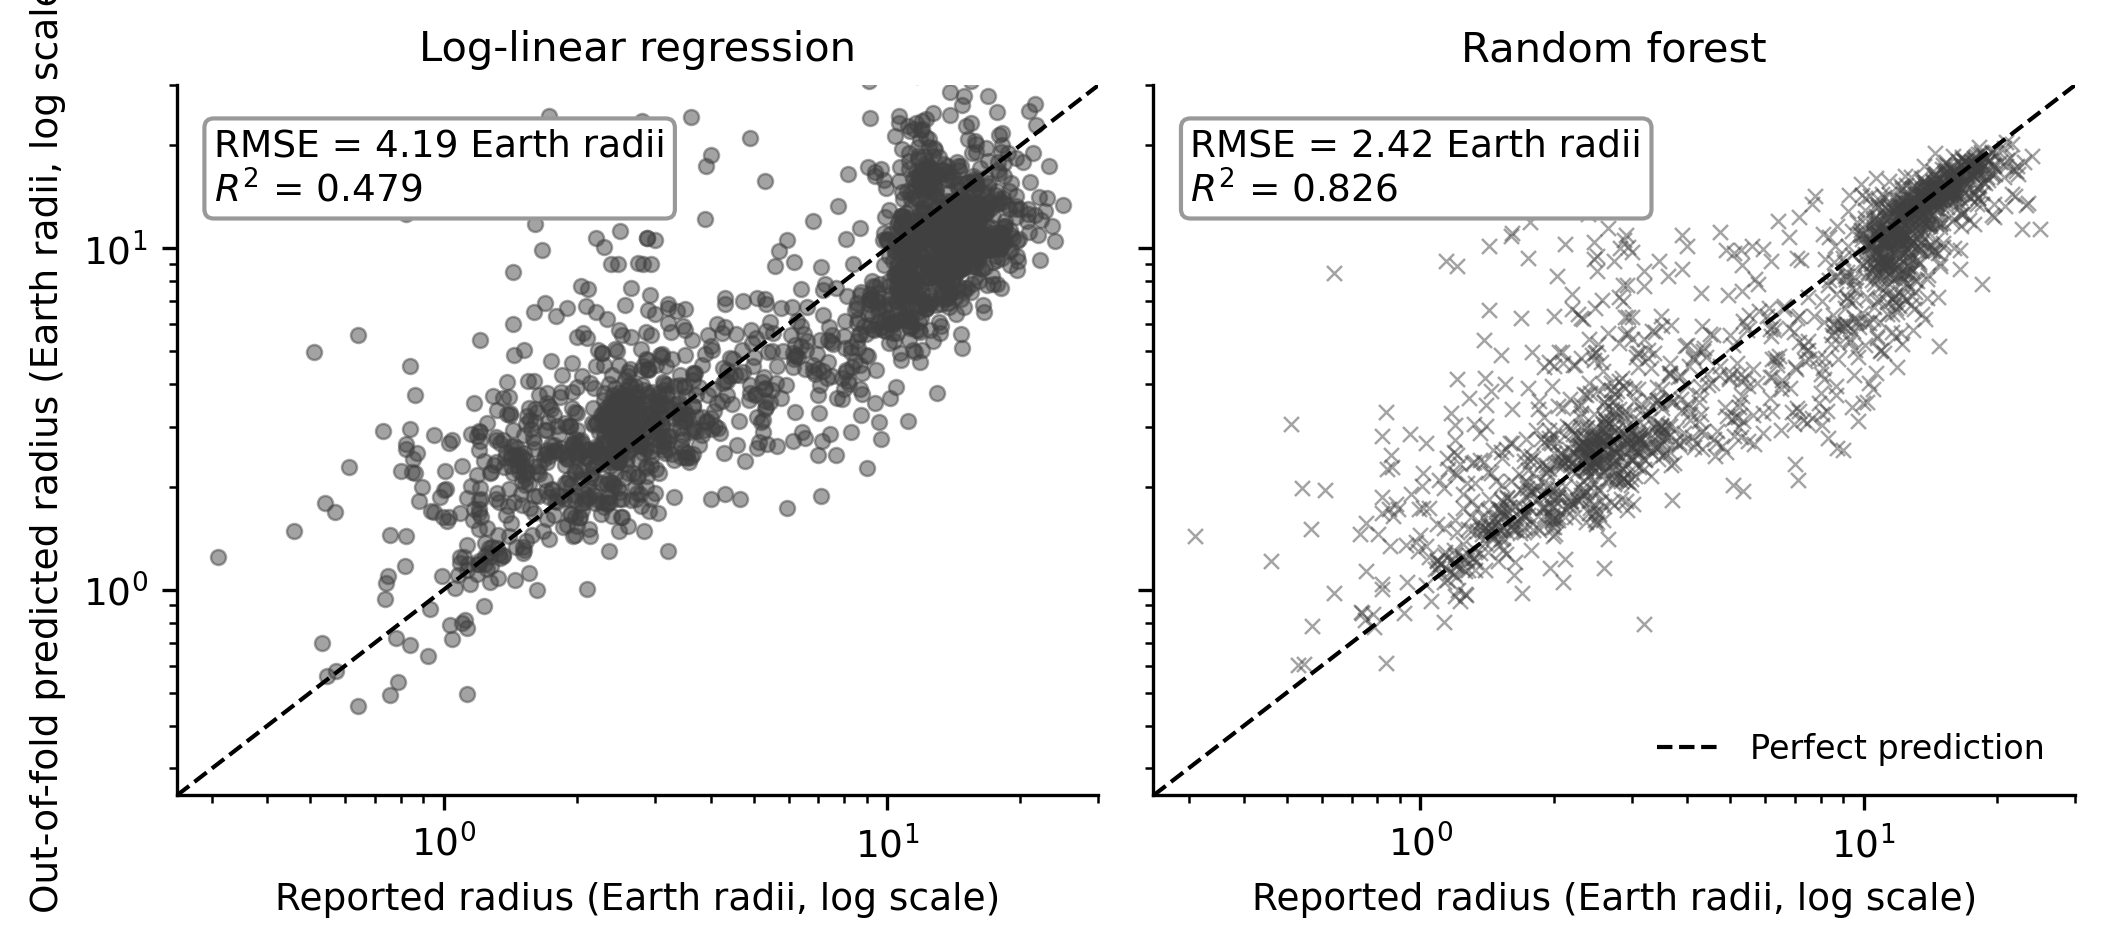
\includegraphics[width=\textwidth]{figures/model_predictions.pdf}
  \caption{Reported and out-of-fold predicted radii. The dashed line denotes perfect prediction. No planet was predicted by a model trained on that planet or another planet from its host system.}
  \label{fig:predictions}
\end{figure}

Permutation importance reinforced the exploratory result. Shuffling planet mass increased forest log-RMSE by 0.323 dex on average. The corresponding increases were much smaller for equilibrium temperature (0.045), orbital period (0.032), stellar mass (0.009), and stellar metallicity (0.006). Importance measures conditional predictive usefulness, not physical causation. In particular, correlated features can share or substitute for predictive information.

\subsection{How Much Data Is Enough?}

Figure~\ref{fig:learning} shows that model choice mattered more than sample size for the log-linear model. Its mean RMSE was 4.46 Earth radii with about 135 training planets, 4.16 with 339, and 4.18 with 1,336; the plateau indicates functional-form bias that additional rows alone will not fix. Forest RMSE was 2.66, 2.68, 2.53, 2.49, and 2.44 Earth radii at mean training sizes of 135, 339, 670, 997, and 1,336 planets. The small non-monotonic change at the first two sizes is within fold variability, while the overall decline after 339 indicates diminishing but continuing benefit. The present 1,670-planet sample is adequate to distinguish the models and estimate broad relationships. More independently measured masses would still help, especially for small and long-period planets that are underrepresented in the characterized transit sample.

\begin{figure}[tbp]
  \centering
  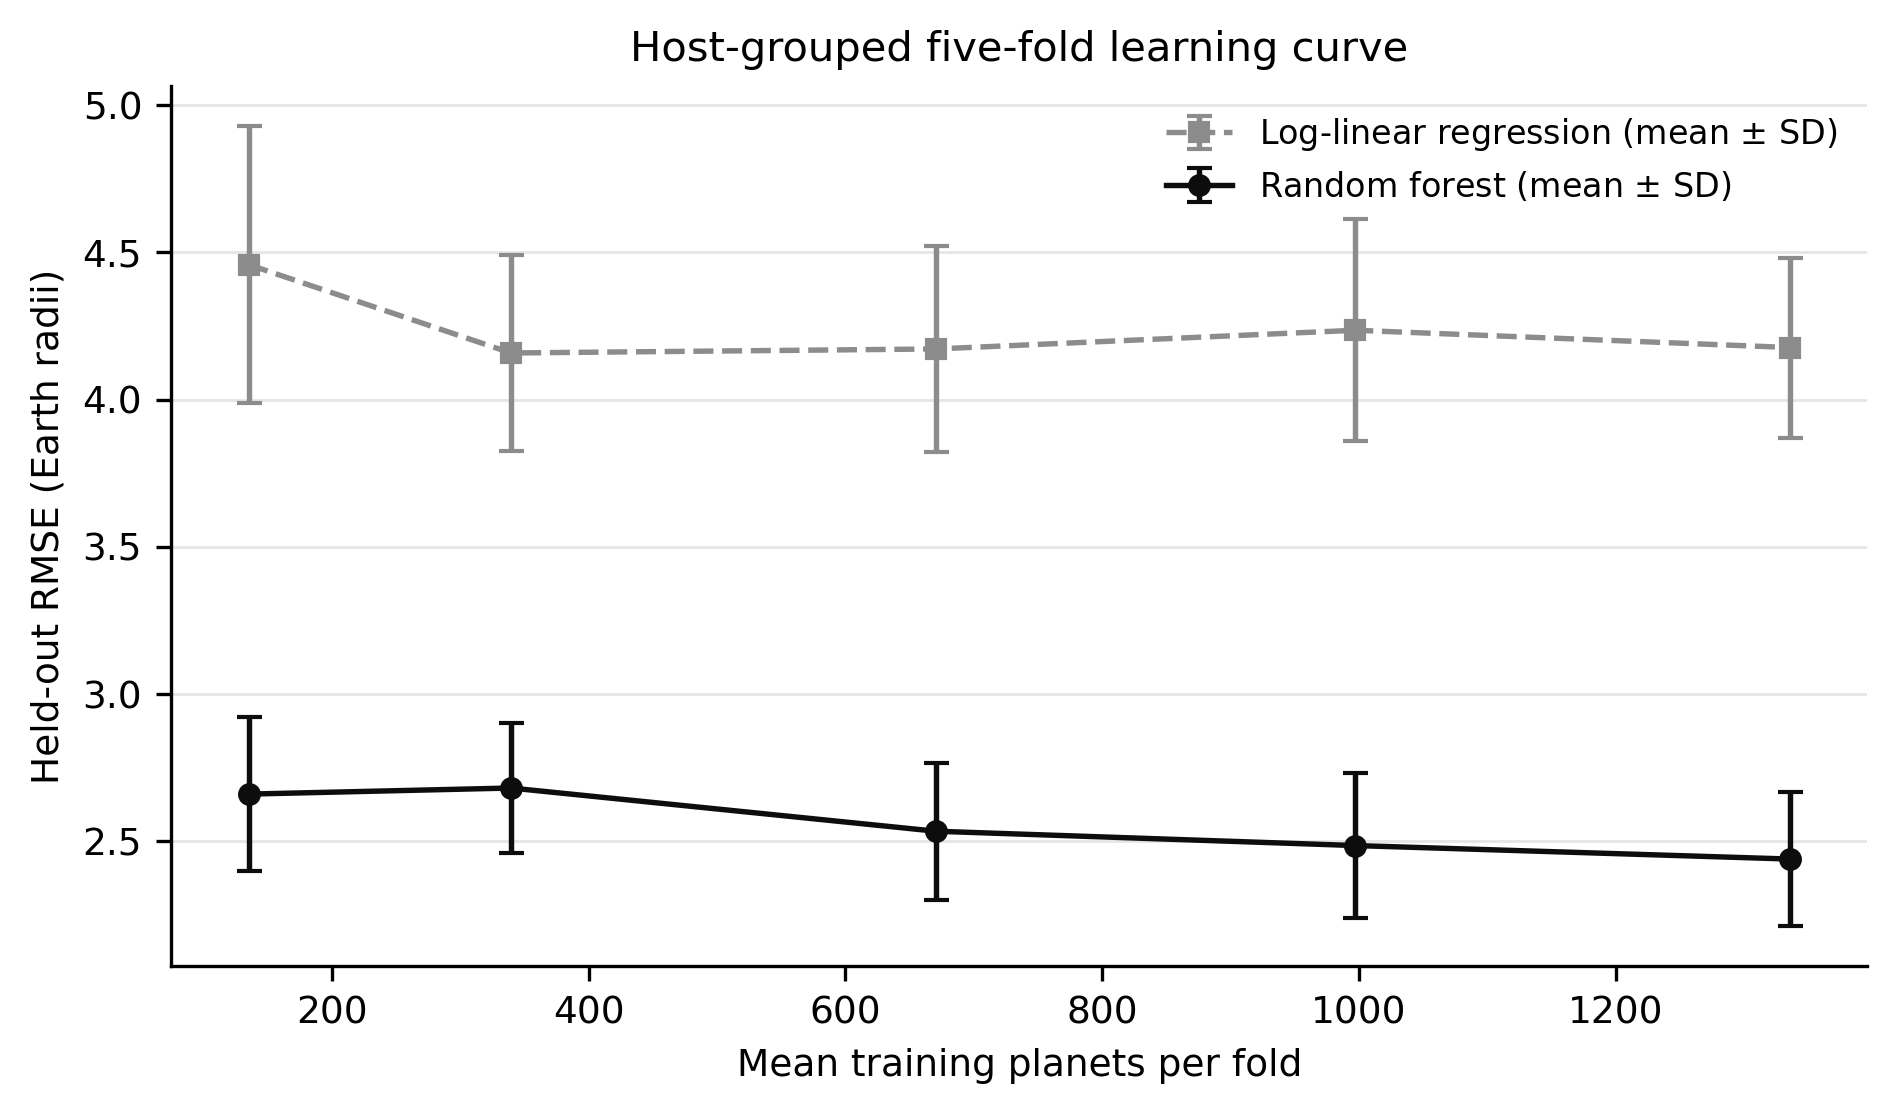
\includegraphics[width=0.86\textwidth]{figures/learning_curve.pdf}
  \caption{Held-out prediction error as host-grouped training data increase. Error bars are standard deviations across five folds; markers and line styles remain distinguishable in grayscale.}
  \label{fig:learning}
\end{figure}

\section{Final Discussion}

The results agreed with our main expectation that planet mass would be the most useful predictor, but the strength and shape of the nonlinearity were more pronounced than a single regression equation could capture. The mass--radius curve rose rapidly for smaller planets and flattened among giant planets, and the random forest reduced pooled out-of-fold RMSE from 4.19 to 2.42 Earth radii compared with log-linear regression. Equilibrium temperature and orbital period added useful secondary information, whereas stellar metallicity contributed little conditional predictive information in this sample. The learning curve suggests that 1,670 planets are enough for a reliable comparison of these two model classes, although additional independently measured masses could still improve the nonlinear model modestly. The conclusions are most applicable to transiting planets similar to those already characterized, not to all exoplanets. Transit detection favors short-period systems, and obtaining an independent mass requires additional observations, creating further selection. Reported catalog values also have unequal measurement uncertainty, which this exercise did not model. Generality would improve with uncertainty-aware regression, a larger sample of small and long-period planets, and external validation on planets added after the snapshot date. Our strongest conclusion is therefore predictive and conditional: within this selected catalog population, mass and nonlinear structure are essential for estimating radius.

\section{Reproducibility and Presentation}

The submission includes the exact archive CSV, TAP query, checksum, analysis code, processed model sample, fold-level results, and figures. Running \texttt{python3 analysis.py} regenerates all numerical outputs with seed 2202; \texttt{latexmk -pdf II2202-quantitative-exercise.tex} rebuilds this report. Figures are stored as vector PDFs for lossless magnification and as 300 dpi PNG files. They use hollow markers, distinct line styles, grayscale contrast, and direct labels rather than color alone.

\bibliographystyle{plainnat}
\bibliography{II2202-quantitative-exercise}

\end{document}
